%\thispagestyle{myheadings}
\newpage
\section{Keynote Speaker: Veronica Perez Rosas}
\setheaders{Keynote Speaker}{\daydateyear}
\index{Perez Rosas, Veronica}

\begin{center}
{\bfseries\Large NLP for Timely and Actionable Feedback\\\vspace{2.0\lineskip}in Healthcare Conversations} \\
\vspace{1.0em}
{\large\bf Veronica Perez Rosas} \\
University of Michigan

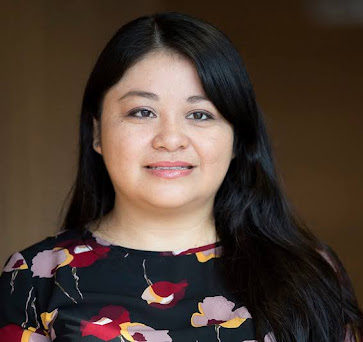
\includegraphics[width=0.4\linewidth]{content/mexican_nlp/veronica.png}

\textbf{\daydateyear{}, 15:30--16:30 CST}\\
\textbf{Do\~na Adelita}
\end{center}

\noindent
{\bfseries Abstract:}
Effective communication is essential in mental healthcare, as it influences patient responses, treatment decisions, and outcomes. In this presentation, I'll discuss computational methods aimed at helping clinicians enhance their communication skills during patient interactions, with a particular focus on feedback and coaching in counseling. Firstly, I'll explore the generation of language cues to assist counselors in crafting responses that align with counseling guidelines, using language models augmented with context and common sense. Secondly, I will introduce language-based coaching systems that use contrastive learning and language models for response scoring and rewriting. These tools aim to empower clinicians to refine their communication skills by providing detailed feedback and enabling them to adapt their style to better suit patients' needs. Finally, I'll share a case study demonstrating the application of these tools in educational settings, highlighting the potential of AI in mental healthcare.

\vspace{1em}

{\bfseries Biography:}
Veronica Perez Rosas is an Assistant Research Scientist at the University of Michigan. Her research interests include Natural Language Processing, Machine Learning, Affect Recognition, and Multimodal Processing of Human Behavior. Her research focuses on developing computational methods to analyze, recognize, and predict human behaviors during social interactions. She has authored papers in leading conferences and journals in Natural Language Processing and Multimodal Processing, has mentored numerous students in these research areas, and has served as workshop chair or area chair for multiple international conferences in the field.

\newpage
